% 2-15-rb-tree.tex

%%%%%%%%%%%%%%%%%%%%
\documentclass[a4paper, justified]{tufte-handout}

% hw-preamble.tex

% geometry for A4 paper
% See https://tex.stackexchange.com/a/119912/23098
\geometry{
  left=20.0mm,
  top=20.0mm,
  bottom=20.0mm,
  textwidth=130mm, % main text block
  marginparsep=5.0mm, % gutter between main text block and margin notes
  marginparwidth=50.0mm % width of margin notes
}

% for colors
\usepackage{xcolor} % usage: \color{red}{text}
% predefined colors
\newcommand{\red}[1]{\textcolor{red}{#1}} % usage: \red{text}
\newcommand{\blue}[1]{\textcolor{blue}{#1}}
\newcommand{\teal}[1]{\textcolor{teal}{#1}}

\usepackage{todonotes}

% heading
\usepackage{sectsty}
\setcounter{secnumdepth}{2}
\allsectionsfont{\centering\huge\rmfamily}

% for Chinese
\usepackage{xeCJK}
\usepackage{zhnumber}
\setCJKmainfont[BoldFont=FandolSong-Bold.otf]{FandolSong-Regular.otf}

% for fonts
\usepackage{fontspec}
\newcommand{\song}{\CJKfamily{song}} 
\newcommand{\kai}{\CJKfamily{kai}} 

% To fix the ``MakeTextLowerCase'' bug:
% See https://github.com/Tufte-LaTeX/tufte-latex/issues/64#issuecomment-78572017
% Set up the spacing using fontspec features
\renewcommand\allcapsspacing[1]{{\addfontfeature{LetterSpace=15}#1}}
\renewcommand\smallcapsspacing[1]{{\addfontfeature{LetterSpace=10}#1}}

% for url
\usepackage{hyperref}
\hypersetup{colorlinks = true, 
  linkcolor = teal,
  urlcolor  = teal,
  citecolor = blue,
  anchorcolor = blue}

\newcommand{\me}[4]{
    \author{
      {\bfseries 姓名:}\underline{#1}\hspace{2em}
      {\bfseries 学号:}\underline{#2}\hspace{2em}\\[10pt]
      {\bfseries 评分:}\underline{#3\hspace{3em}}\hspace{2em}
      {\bfseries 评阅:}\underline{#4\hspace{3em}}
  }
}

% Please ALWAYS Keep This.
\newcommand{\noplagiarism}{
  \begin{center}
    \fbox{\begin{tabular}{@{}c@{}}
      请独立完成作业,不得抄袭。\\
      若得到他人帮助, 请致谢。\\
      若参考了其它资料,请给出引用。\\
      鼓励讨论,但需独立书写解题过程。
    \end{tabular}}
  \end{center}
}

\newcommand{\goal}[1]{
  \begin{center}{\fcolorbox{blue}{yellow!60}{\parbox{0.50\textwidth}{\large 
    \begin{itemize}
      \item 体会``思维的乐趣''
      \item 初步了解递归与数学归纳法 
      \item 初步接触算法概念与问题下界概念
    \end{itemize}}}}
  \end{center}
}

% Each hw consists of four parts:
\newcommand{\beginrequired}{\hspace{5em}\section{作业 (必做部分)}}
\newcommand{\beginoptional}{\section{作业 (选做部分)}}
\newcommand{\beginot}{\section{Open Topics}}
\newcommand{\begincorrection}{\section{订正}}
\newcommand{\beginfb}{\section{反馈}}

% for math
\usepackage{amsmath, mathtools, amsfonts, amssymb}
\newcommand{\set}[1]{\{#1\}}

% define theorem-like environments
\usepackage[amsmath, thmmarks]{ntheorem}

\theoremstyle{break}
\theorempreskip{2.0\topsep}
\theorembodyfont{\song}
\theoremseparator{}
\newtheorem{problem}{题目}[subsection]
\renewcommand{\theproblem}{\arabic{problem}}
\newtheorem{ot}{Open Topics}

\theorempreskip{3.0\topsep}
\theoremheaderfont{\kai\bfseries}
\theoremseparator{:}
\theorempostwork{\bigskip\hrule}
\newtheorem*{solution}{解答}
\theorempostwork{\bigskip\hrule}
\newtheorem*{revision}{订正}

\theoremstyle{plain}
\newtheorem*{cause}{错因分析}
\newtheorem*{remark}{注}

\theoremstyle{break}
\theorempostwork{\bigskip\hrule}
\theoremsymbol{\ensuremath{\Box}}
\newtheorem*{proof}{证明}

% \newcommand{\ot}{\blue{\bf [OT]}}

% for figs
\renewcommand\figurename{图}
\renewcommand\tablename{表}

% for fig without caption: #1: width/size; #2: fig file
\newcommand{\fig}[2]{
  \begin{figure}[htbp]
    \centering
    \includegraphics[#1]{#2}
  \end{figure}
}
% for fig with caption: #1: width/size; #2: fig file; #3: caption
\newcommand{\figcap}[3]{
  \begin{figure}[htbp]
    \centering
    \includegraphics[#1]{#2}
    \caption{#3}
  \end{figure}
}
% for fig with both caption and label: #1: width/size; #2: fig file; #3: caption; #4: label
\newcommand{\figcaplbl}[4]{
  \begin{figure}[htbp]
    \centering
    \includegraphics[#1]{#2}
    \caption{#3}
    \label{#4}
  \end{figure}
}
% for margin fig without caption: #1: width/size; #2: fig file
\newcommand{\mfig}[2]{
  \begin{marginfigure}
    \centering
    \includegraphics[#1]{#2}
  \end{marginfigure}
}
% for margin fig with caption: #1: width/size; #2: fig file; #3: caption
\newcommand{\mfigcap}[3]{
  \begin{marginfigure}
    \centering
    \includegraphics[#1]{#2}
    \caption{#3}
  \end{marginfigure}
}

\usepackage{fancyvrb}

% for algorithms
\usepackage[]{algorithm}
\usepackage[]{algpseudocode} % noend
% See [Adjust the indentation whithin the algorithmicx-package when a line is broken](https://tex.stackexchange.com/a/68540/23098)
\newcommand{\algparbox}[1]{\parbox[t]{\dimexpr\linewidth-\algorithmicindent}{#1\strut}}
\newcommand{\hStatex}[0]{\vspace{5pt}}
\makeatletter
\newlength{\trianglerightwidth}
\settowidth{\trianglerightwidth}{$\triangleright$~}
\algnewcommand{\LineComment}[1]{\Statex \hskip\ALG@thistlm \(\triangleright\) #1}
\algnewcommand{\LineCommentCont}[1]{\Statex \hskip\ALG@thistlm%
  \parbox[t]{\dimexpr\linewidth-\ALG@thistlm}{\hangindent=\trianglerightwidth \hangafter=1 \strut$\triangleright$ #1\strut}}
\makeatother

% for footnote/marginnote
% see https://tex.stackexchange.com/a/133265/23098
\usepackage{tikz}
\newcommand{\circled}[1]{%
  \tikz[baseline=(char.base)]
  \node [draw, circle, inner sep = 0.5pt, font = \tiny, minimum size = 8pt] (char) {#1};
}
\renewcommand\thefootnote{\protect\circled{\arabic{footnote}}} % feel free to modify this file
%%%%%%%%%%%%%%%%%%%%
\title{第15讲: 红黑树}
\me{林凡琪}{211240042}{}{}
\date{\zhtoday} % or like 2019年9月13日
%%%%%%%%%%%%%%%%%%%%
\begin{document}
\maketitle
%%%%%%%%%%%%%%%%%%%%
\noplagiarism % always keep this line
%%%%%%%%%%%%%%%%%%%%
\begin{abstract}
  % \begin{center}{\fcolorbox{blue}{yellow!60}{\parbox{0.65\textwidth}{\large 
  %   \begin{itemize}
  %     \item 
  %   \end{itemize}}}}
  % \end{center}
\end{abstract}
%%%%%%%%%%%%%%%%%%%%
\beginrequired

%%%%%%%%%%%%%%%
\begin{problem}[TC 18.1-5]
\end{problem}

\begin{solution}
  在将每个红色节点吸收到其黑色父节点之后,每个黑色节点可能包含 $1、2$($1$ 红色子节点)或 $3$($2$ 红色子节点)键,并且结果树的所有叶子都具有相同的深度,根据到红黑树的性质5(对于每个节点,从节点到后代叶子的所有路径都包含相同数量的黑色节点)。 因此,红黑树会变成度数$t = 2$的Btree,即2-3-4树。
\end{solution}
%%%%%%%%%%%%%%%

%%%%%%%%%%%%%%%
\begin{problem}[TC 13.1-5]
\end{problem}

\begin{solution}
  是的。\\
  性质一很容易满足,因为之更改了一个节点,并且没有更改为第三种颜色;\\
  性质三也很容易满足,因为没有引入新的叶子节点;\\
  性质四被满足,因为没有引入红色节点,对这条性质没有影响;\\
  性质五被满足,因为我们将更改黑色节点数量的唯一路径是来自根的路径.所有的路径上的黑色节点都将增加1,因此是平等的.
\end{solution}
%%%%%%%%%%%%%%%

%%%%%%%%%%%%%%%
\begin{problem}[TC 13.1-7]
\end{problem}

\begin{solution}
  可能的degree是 $0$ 到 $5$,这取决于黑色节点是否是根以及它是有一个还是两个红色子节点。深度最多可以缩小 $1 / 2$ 倍。
\end{solution}
%%%%%%%%%%%%%%%

%%%%%%%%%%%%%%%
\begin{problem}[TC 13.3-1]
\end{problem}

\begin{solution}
  如果我们选择将 $z$ 的颜色设置为黑色,那么我们将违反作为红黑树的性质5。 因为从根到 $z$下的叶子的任何路径都会比到其他叶子的路径多一个黑色节点。
\end{solution}
%%%%%%%%%%%%%%%

%%%%%%%%%%%%%%%
\begin{problem}[TC 13.3-5]
\end{problem}

\begin{solution}
  情形1:$z$和$z.p.p$是$\text{RED}$,如果循环终止,那么$z$不可能是根,因此修复后$z$是$\text{RED}$ .\\
  情形2:$z$和$z.p$是$\text{RED}$,旋转后$z.p$不可能是根,因此修复后$z.p$是$\text{RED}$。\\
  情形3:$z$ 是 $\text{RED}$ 并且$z$不能是根,因此修复后$z$是$\text{RED}$。
  因此,总是至少有一个红色节点。
\end{solution}
%%%%%%%%%%%%%%%

%%%%%%%%%%%%%%%
\begin{problem}[TC 13.4-1]
\end{problem}

\begin{solution}
  情形1:转换为2、3、4。
  情形2:如果终止,则子树的根(新的 $x$)设置为黑色。
  情形3:转换为 4。
  情形4:根(即新的 $x$)设置为黑色。
\end{solution}
%%%%%%%%%%%%%%%

%%%%%%%%%%%%%%%
\begin{problem}[TC 13.4-7]
\end{problem}

\begin{solution}
  不一定和原来一样.\\
  比如:\\
  原红黑树树如图:\\
  \begin{figure}
    \centering
    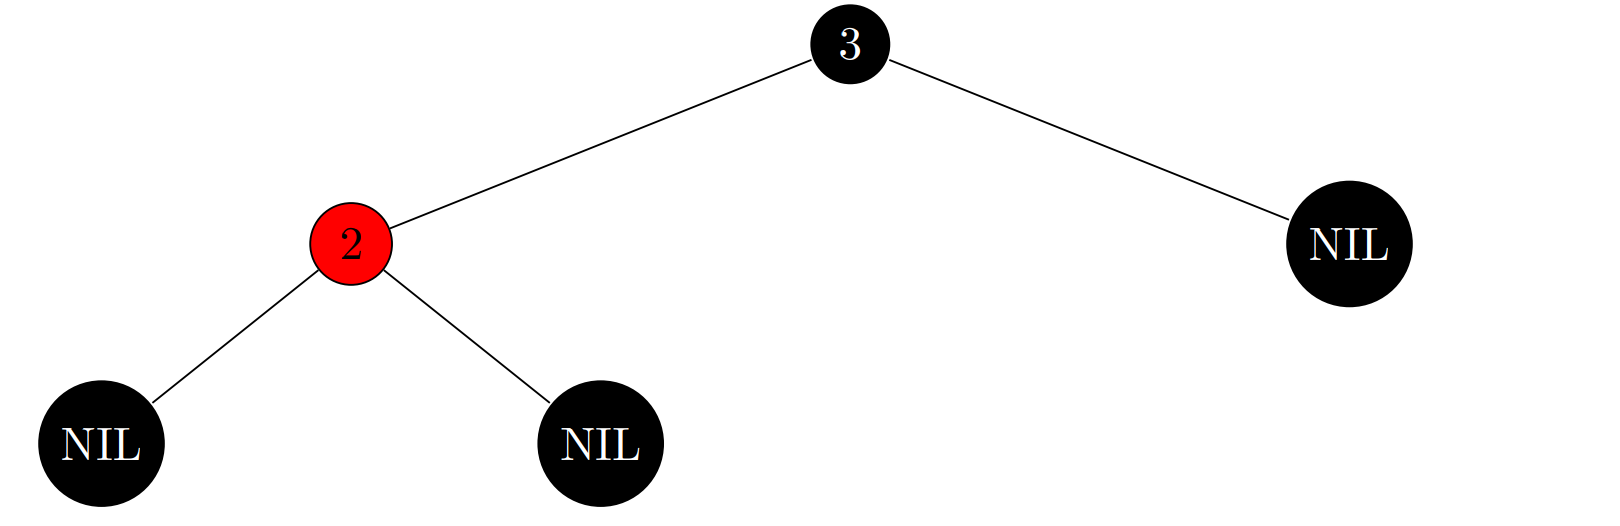
\includegraphics[width=10cm,height=5cm]{pic1.png}
  \end{figure}
  插入1后:
  \begin{figure}
    \centering
    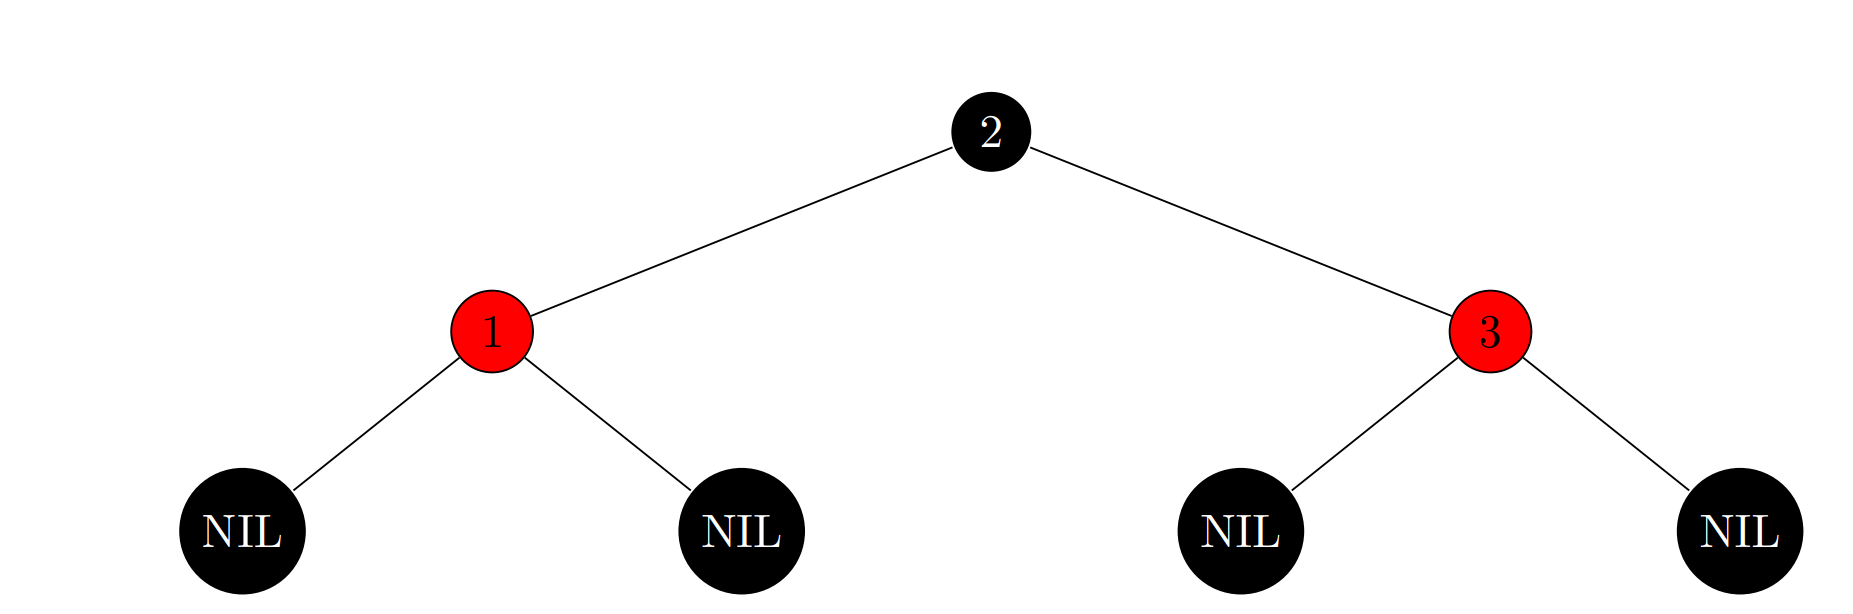
\includegraphics[width=10cm,height=5cm]{pic2.png}
  \end{figure}
  删除1后:
  \begin{figure}
    \centering
    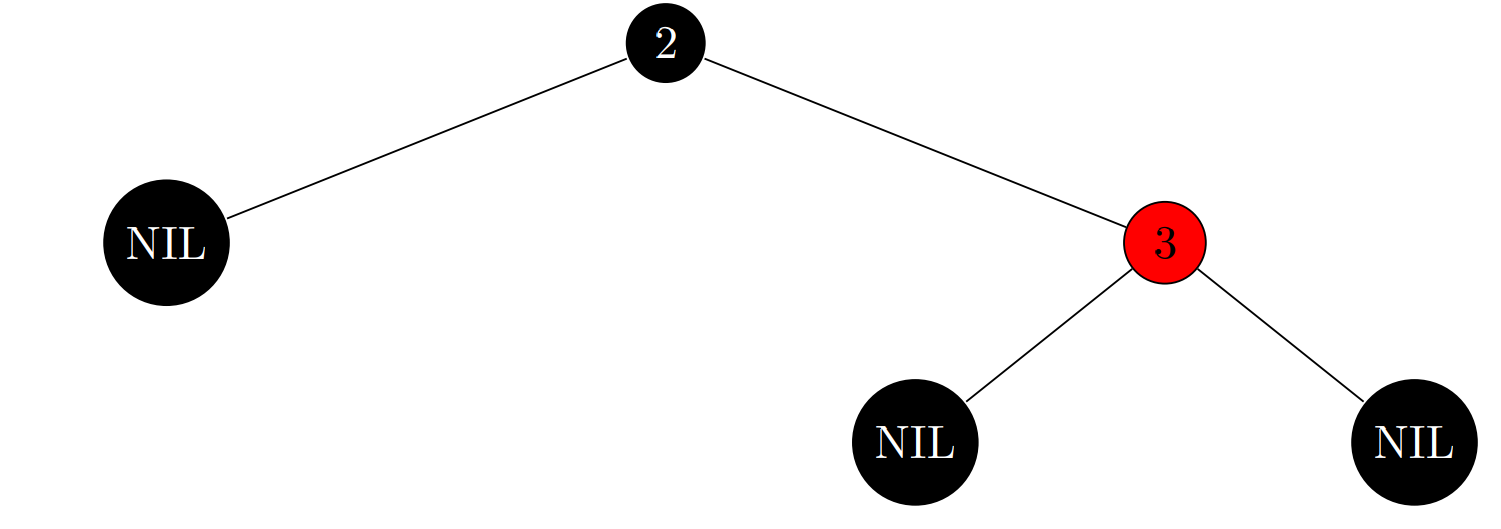
\includegraphics[width=10cm,height=5cm]{pic3.png}
  \end{figure}
  显然,最后和刚开始不同.
\end{solution}
%%%%%%%%%%%%%%%

%%%%%%%%%%%%%%%%%%%%
\beginoptional

%%%%%%%%%%%%%%%
\begin{problem}[TC Problem 13-3: AVL trees]
\end{problem}

\begin{solution}
\end{solution}
%%%%%%%%%%%%%%%

%%%%%%%%%%%%%%%%%%%%
\beginot

%%%%%%%%%%%%%%%
% \begin{ot}[]
% \end{ot}

% \begin{solution}
% \end{solution}
%%%%%%%%%%%%%%%
% \vspace{0.50cm}
%%%%%%%%%%%%%%%
% \begin{ot}[]
% 
%   \noindent 参考资料:
%   \begin{itemize}
%     \item 
%   \end{itemize}
% \end{ot}

% \begin{solution}
% \end{solution}
%%%%%%%%%%%%%%%

%%%%%%%%%%%%%%%%%%%%
% 如果没有需要订正的题目,可以把这部分删掉

\begincorrection
\begin{problem}[$D_{n}$1-13.2]
请证明: $D_{n}$ (定义见阅读材料 Example 15.1 (c))
是 Boolean algebra 当且仅当 $n = p_1 p_2 \cdots p_k$ (for some $k$),
这里 $p_i$ 皆为素数且互异。
\end{problem}

\begin{solution}
  Suppose, to the contrary. There exists  Boolean algebra $D_{n}= p_1^{t_1} p_2^{t_2} \cdots p_k^{t_k}$(for some $k$, and $t_{i}\in \mathbb{N^{+}}$) satisfied these $p_i$ are all different prime numbers but $t_{i}$ are not all 1.\\
  Assume that $t_1\neq 1$.\\
  Let $a=p_1$, and $a^{\prime}= p_1^{t_1-1} p_2^{t_2} \cdots p_k^{t_k}$.\\
  So we can have that $a*a^{\prime}=gcd(a,a^{\prime})=p_1$\\
  With the definition, $a*a^{\prime}=1$ but $p_1\neq 1$, which $1$ is the zero element.\\
  It is contradict with the definition of Boolean algebra.\\
  So if $D_{n}$ is Boolean algebra, then $n = p_1 p_2 \cdots p_k$ (for some $k$), and  these $p_i$ are all different prime numbers. \hfill(1)\\
  If $D_{n}$ satisfied $n = p_1 p_2 \cdots p_k$ (for some $k$), and  these $p_i$ are all different prime numbers,  then $D_{n}$ is a Boolean algebra as the textbook SM explained.\hfill(2)\\
  $(1)\land (2)\to$ $D_{n}$ is Boolean algebra if and only if $n = p_1 p_2 \cdots p_k$ (for some $k$), and  these $p_i$ are all different prime numbers.
\end{solution}

\begin{problem}[2-1.5 DH Problem $5.14\; (a, b)$: $\textsl{Pal4}(S)$]
Note: You don't have to consider $\textsl{Pal3}$ in Problem $5.13$.\\
(a)Construct a correct solution to the problem of checking efficiently whether a string is
a palindrome, following the general ideas of Pal2 and Pal3. Call your algorithm Pal4.\\
(b) Prove the total correctness of Pal4.\\
\end{problem}

\begin{solution}
  (a)\\
  \noindent
  \begin{algorithm}
    \begin{algorithmic}[1]
      \caption{judge whether the string is a palindrome}\label{euclid}
      \Procedure{Pal4}{$S$}
      \State $X\gets S$
      \State $E\gets true$
      \While{$X\neq\boldsymbol{\Lambda}$ and $E==true$}
      \If{\textbf{eq(head($X)$,last($X$))}}
      \State $X\gets \textbf{all-but-last(tail(X))}$
      \Else
      \State $E\gets false$
      \EndIf
      \EndWhile
      \State\Return E
      \EndProcedure
    \end{algorithmic}
  \end{algorithm}

  \noindent(b)\\
  The partially correction has been proven in Problem4(a).\\
  Now we prove the algorithm will terminate.\\
  If the string is not a a palindrome, then line 8 will make E=false in one turn, and the while-do loop will break.\\
  If the string is a palindrome, then every time the while-do loop is traversed, $X$ is made shorter by at most two symbol, and finally becomes $\boldsymbol{\Lambda}$. The while-do loop will break. \\
  Therefore, if the input string is legal, the algorithm will terminate.\\
  Since Pal4 is partially correct and will terminate finally, Pal4 is totally correct.
\end{solution}

\begin{problem}[2-2.4 TC Exercise 3.1-6]
Prove that the running time of an algorithm is \(\Theta(g(n))\) if and only if its worst-case running time is \(O(g(n))\) and its best-case running time is \(\Omega(g(n))\)
\end{problem}

\begin{solution}
  Assume that the running time of the algorithm is $f(n)$.\\
  $f(n)=\Theta(g(n))$\\
  $\leftrightarrow \exists n_0,c_1,c_2,(\forall n,(n\geq n_0\to 0\leq c_1g(n)\leq f(n)\leq c_2g(n)))$\\
  $\leftrightarrow \exists n_0,c_1,c_2,(\forall n,(n\geq n_0\to (0\leq c_1g(n)\leq f(n))\land(0\leq f(n) \leq c_2g(n))))$\\
  $\leftrightarrow f(n)=O(g(n))\land f(n)=\Omega(g(n))$\\
  The $O(g(n))$ describes the upper bound of $f(n)$, and $\Omega(g(n))$ describes the lower bound of $f(n)$.\\
  Therefore, we can have that  the running time of an algorithm is $\Theta(g(n))$ if and only if its worst-case running time is $O(g(n))$ and its best-case running time is $\Omega(g(n))$.
\end{solution}

\begin{problem}[2-4.4 TC 4.5-4]
Can the master method be applied to the recurrence $T(n)=4 T(n / 2)+n^{2} \lg n ?$ Why or why not? Give an asymptotic upper bound for this recurrence.
\end{problem}

\begin{solution}
  The master method can not be used to solve that, since $\frac{n^2\lg n}{n^{\log_2{4}}}=\lg n$ which is not not polynomially larger.\\
  On the  recursion-tree, The depth is  $log_2{n}+1$, and the total cost is  $n^2log_2n-n^2i$ nodes in the $i^{th}$ depth.\\
  $\sum\limits_{i=0}^{\log_2n}n^2log_2n-n^2i=O(\sum\limits_{i=0}^{\log_2n}n^2log_2n)$\\
  Therefore, $T(n)=O(n^2log^2n)$.
\end{solution}

\begin{problem}[2-6.1 DH 4-8]
Prove that the maximal distance between any two points on a polygon occurs between two of the vertices.
\end{problem}

\begin{solution}
  对于在凸包上的任意两点,我们一定可以分别过这两个点做直线,满足两条直线平行,且直线间距离等于两点间距离。\\
  将这两条直线分别向外平移。对于每条直线,当他仅经过凸包上的一个顶点,或恰好包含凸包上的一条边时停止平移。\\
  此时显然有平移后直线间距离大于等于原来选取的两点间距离。\\
  此时分为3种情况:\\
  1, 若平移后两条直线都恰好经过凸包的一个顶点,显然有两顶点距离大于等于直线间距离。因此两顶点距离大于等于原选点距离。得证。\\
  2, 若平移后恰好有一条直线包含凸包上的一条边,显然有另一条直线所经过的顶点,到这条边两个顶点的距离最大值,大于等于原选点距离。得证。\\
  3, 若平移后两条直线都包含凸包上的边,显然有这两条边的四个顶点间的距离最大值,大于等于原选点距离。得证。\\
  综上,在凸包中选取任意两点,都能找到凸包上的两个顶点,满足顶点间距离大于等于所选点。\\
  原命题得证。
\end{solution}

\begin{problem}[2-6.3 DH 4-12]
Write high-level pseudocode of the greedy algorithm described in the text
for finding a minimal spanning tree.
\end{problem}

\begin{solution}
  \begin{algorithm}
    \caption{minimal spanning tree}\label{euclid}
    \begin{algorithmic}[1]
      \Procedure{cost}{A[],n}
      \Comment{A为一组有连边关系的点的二元组,n为组数}
      \State $ans \to 0$
      \State sort(A)\Comment{将二元组按花费从小到大的顺序排序}
      \For {$i\gets 1$ to $n$}
      \If{is\_connected(A[i].x,A[i].y)==False}
      \State connext A[i].x and A[i].y
      \State $ans\to ans+A[i].cost$
      \EndIf
      \EndFor
      \State \Return ans
      \EndProcedure
    \end{algorithmic}
  \end{algorithm}

\end{solution}

\begin{problem}[2-15.2 TC 13.1-7]
Describe a red-black tree on $n$ keys that realizes the largest possible ratio of red internal nodes to black internal nodes. What is this ratio? What tree has the smallest possible ratio, and what is the ratio?
\end{problem}

\begin{solution}
  (1)\\
  当红黑树中满足:每个黑色节点的子节点若不为nil,则为红节点  时,其内节点的红黑比最大。\\
  若$n=2^{2k}-1$,$k\in \mathbb{N^+}$时,红黑树全黑节点层与全红节点层交替出现,此时最大红黑比为2\\
  (2)\\
  当红黑树中所有内节点都为黑色节点时,其红黑比最小,为0.
\end{solution}

\begin{problem}[2-15.3 TC 13.3-1]
In line 16 of $\mathrm{RB}$ -INSERT, we set the color of the newly inserted node $z$ to red. Observe that if we had chosen to set $z$ 's color to black, then property 4 of a redblack tree would not be violated. Why didn't we choose to set $z$ 's color to black?
\end{problem}

\begin{solution}
  将节点设为红色,会破坏性质2/4,调整这一后果影响的节点较为局限,便于操作\\
  若将节点设为黑色,性质5则会被破坏。若从维护性质5的角度去解决,问题会变得更加棘手
\end{solution}
%%%%%%%%%%%%%%%%%%%%

%%%%%%%%%%%%%%%%%%%%
% 如果没有反馈,可以把这部分删掉
\beginfb

% 你可以写
% ~\footnote{优先推荐 \href{problemoverflow.top}{ProblemOverflow}}:
% \begin{itemize}
%   \item 对课程及教师的建议与意见
%   \item 教材中不理解的内容
%   \item 希望深入了解的内容
%   \item $\cdots$
% \end{itemize}
%%%%%%%%%%%%%%%%%%%%
% \bibliography{2-5-solving-recurrence}
% \bibliographystyle{plainnat}
%%%%%%%%%%%%%%%%%%%%
\end{document}